\chapter{Constrained Geometric Approximation}
\label{chp:cga}

In this chapter, we focus on the planning problem for the robot subject to bounded
motion and sensing uncertainty.

The idea of representing and eliminating the uncertainty in a range space is inspired by O'Kane's
work~\cite{OKa11}. The author solved a decentralized tracking problem by letting
robots maintain proximity to a collection of unpredictably moving targets using
low-resolution sensors. Similarly, we over-approximate a robot's information state 
by constraining the geometric operations to produce sets within the range space. 
Our contributions stated in this chapter include new operations defined for the range space 
and the algorithm carrying out those operations. 

We organize the remaining of this chapter as following: in Section~\ref{sec:related-cga}, 
we review prior research related to our work. 
%
We define the problem formulation and describe the robot model as well as the
fundamental notations related to the information space in Section~\ref{sec:robot-mod} and Section~\ref{sec:ispace}. 
In Section~\ref{sec:rspace}, we define two operations
associated with the range space and discuss about the constrained geometric
approximation algorithm in detail. In Section~\ref{sec:simu-cga}, we provide groups of
experiments and collect the simulation results to evaluate the performance of our method
using different landmark-based navigation tasks. 
Based on the measurements of the computation time and the approximation quality of the algorithm
against three types of range spaces, we draw conclusions of our approach in the last section.

%\clearpage
\section{Related Work}
\label{sec:related-cga}
Most of prior work in robotics research community represented and reasoned about
the robot's uncertainty using probabilistic models. Especially for the
robot's navigation, simultaneous localization and mapping (SLAM), and searching problems, etc.,
the probabilistic approaches are well studied and widely used \cite{ThrBurFox98,
  ThrBurFox00, ThrBurFox05,JenKri01,SimKoe95,ThrBee+00,
  TomYut01,KamManMin96}. 
Thrun, Burgard, and Fox developed an algorithm for
landmark-based localization and mapping in the indoor environments where
the landmarks' locations and robot's positions are estimated by a likelihood
maximized under probabilistic constraints~\cite{ThrBurFox98}. In their work, the
probabilistic models were used to represent and reason about both of robot's
sensing and motion. 
Bayesian estimation algorithms were also used in Thrun's
work~\cite{Thr01} to estimate the robots' states from sensor measurements,
in order to conduct the concurrent mapping and localization tasks. 
Simmons and Koenig developed a navigation approach based on the partially observable Markov models
to track the location of the robot and maintains a probability distribution over all
possible locations with sensing and motion uncertainty~\cite{SimKoe95}.
Jensfelt and Kristensen solved a global localization problem using
probabilistic approach based on the topological world models, in which a Kalman
filter~\cite{Kal60} was applied to represent and track a number of pose
hypotheses of the robot~\cite{KuiByu91}. 

More recent work has used such probabilistic representations explicitly for
motion planning~\cite{KufLav00,PepKieWal09,BerAbbGol11,PreRoy09}. 
Kuffner and LaValle proposed a probabilistically complete randomized data structure called
rapidly-exploring random tree (RRT) for path planning~\cite{KufLav00}.  
Pepy, Kieffer, and Walter addressed the path planning problem by combining RRT and the set
representation of states with bounded uncertainty, they developed a ``Box-RRT'' path
planner and applied the method to nonholonomic vehicles. 
Berg, Abbeel and Goldberg presented a linear-quadratic Gaussian motion planning (LQG-MP) algorithm that
based on the linear-quadratic controller with Gaussian models of motion and
sensing noise~\cite{BerAbbGol11}. 
Prentice and Roy presented a planning algorithm for the linear Gaussian systems in belief (information) space to compute the reachable belief (information) state and find the path with minimum
expected cost, by reducing the computational cost of the extended Kalman filter
predictions~\cite{PreRoy09}.

The probabilistic approaches, including but not limited to above-mentioned work,
demonstrated considerable success in solving SLAM, navigation, and path planning problems. 
However, probabilistic methods are often computationally expensive. 
For example, Kavraki, Svestka, Latombe and Overmars presented an approach to construct the probabilistic roadmap in the high-dimensional collision-free configuration spaces~\cite{KavSve+96}. 
This technique may require the connections of thousands of configurations or states
to find a solution.
Another example is the usage of the Monte Carlo methods for localization problems:
the particle filters is often implemented with hundreds or thousands of particles~\cite{ThrFox+00}. 
Therefore, these approaches could be impractical for robots with limitations of computing power.

Moreover, another fact that limits the usage of probabilistic methods is that it
is difficult for the robot to decide how sufficiently many particles are
necessary to guarantee the convergence to the correct solution, based on a
realistic consideration of maintaining a relative small number of particles. 

Motivated by the idea of finding approach fitted to the robot applications 
with extreme limited computational capability, we developed a method
to maintain a set of the over-approximation of true information state, in
contrast to the particle filtering. 
Therefore, the robot can directly determine when the information it represents 
is not useful because of the insufficient detail of true I-state.

Another branch of robotics research, which has described itself as a ``minimalist''
approach, for example, following algorithms solved the problems in spite of limitations
in the robot's sensing capability~\cite{AkeMas98,Erd86, % manipulation
  KamRiv97, LumTiw94,BluRagSch97,LazLat92, %navigation
  TovGuiLav04, AcaCho01b,ChoBur00}. %mapping}.
Akella and Mason introduced a classification of polygonal objects subject to
linear pushing actions. They described a complete pose planner to
construct a sequence of pushing actions to move a polygonal object from any
initial pose to any final pose regardless of the feedback sensing~\cite{AkeMas98}. 
%
Kamon and Rivlin presented a planning algorithm using the range data, 
this approach ensures to navigate the robot to reach the target in an unknown environment or to report the target is unreachable~\cite{KamRiv97}. 
%
Lazanas and Latombe described a complete polynomial algorithm to solve a navigation
problem in spite of uncertainty. 
%
Given landmarks scattered across the environment, the planner computes a plan with bounded uncertainty by
backtracking the omnidirectional back-projections of the goal, until one fully
contains the set of possible initial positions of the robot~\cite{LazLat92}.
%
Tovar, Guilamo and LaValle presented a data structure of the ``Gap Navigation Tree''
(GNT) to solve different visibility-based tasks with minimal sensing requirements in unknown planar environments, 
whose boundaries were piecewise smooth closed curves, with finite number of non-smooth points~\cite{TovGuiLav04}. 
The GNT structure reflects the path information in the information space, 
it is constructed from the online sensor measurements and updated during the robot's moving. 
%
Tovar, LaValle and Murrieta also showed that robots can complete the tasks such as navigation~\cite{TovLavMur03b}, pursuit-evasion~\cite{TovLav06}, etc., using the GNT approach.
%
Acar, Choset and Atkar conducted work on the sensor-based coverage path planning method to
determine a path that passes a detector, whose range extended beyond the robot's
periphery, over all points in an unknown environment~\cite{AcaCho01b}. 
%
They combined approaches of the sensor-based coverage algorithm~\cite{AcaCho01a,AcaCho00, ChoAcaRizLun00} and the motion planning algorithm used to navigate the robot along the generalized Voronoi diagram~\cite{ChoKonRiz97, ChoBur00} to completely cover an obstacle-free space with an infinite-range
detector. 
%
Tokekar and Isler worked on the problem of placing bearing sensors with bounded uncertainty for robot localization~\cite{TokIsl13}. 
They showed that, given a fixed number of nearby sensors, the robot can localize itself in an unknown environment without losing much estimation quality.

However, these methods generally consider the assumptions of the robot's sensing limitations, 
but not in computation. 
%
In contrast to the complicated procedure of computing the true I-state~\cite{TovLav08, YuLav10}, 
our work contributed to demonstrate that such precise I-states are not always necessary for a robot to complete its task.
Additionally, it is much more efficient to compute reasonable constrained approximations~\cite{SonOka12}.

%\clearpage
\section{Robot Model}
\label{sec:robot-mod}
We consider the point robot in our problem and assume that the robot can not reason about
its state from the observations directly. 
%
Instead, the robot maintains a set of all possible states from its observations. 
%
The robot model contains following concepts in detail.
\begin{enumerate}
\item \emph{State space} $X = \Real^2$: a discrete state space $X$ is
  partitioned into obstacle space $X\sub{obst}$ and obstacle-free space
  $X\sub{free}$. The state of the robot at stage $k \in \Natural$ is written as
  $x_k$.
\item \emph{Action space} $U$: the robot chooses one action $u_k \in U$ which is
  addictive to the state at each stage.
\item \emph{State transition function} $F : X \times U \to \pow(X)$: a
  set-valued transition function is used to describe how does the robot's state $x_k$
  change along with an action $u_k$, with $x_{k+1} \in F(x_k, u_k)$. The
  $\pow(X)$ denotes the powerset of $X$. We consider an addictive noise
  $\theta_k$ to robot's action $u_k$, and we also assume the bounded set of
  uncertainty for a certain action, denote as $\Theta(u_k)$, such that
  \begin{equation}
    \label{eq:state-trans}
    F(x_k, u_k) = \left\{
      x_k + u_k + \theta_k
      \mid
      \theta_k \in \Theta(u_k)
    \right\} \cap X\free.
  \end{equation}
  We assume the bounded noise on both the direction and magnitude of the robot's
  action. 
  The angular noise is bounded by a fixed angle $\delta\sub{ang}$, and
  the translation noise is bounded by $\delta\sub{trans}||u||$. 
  Thus, the
  transition noise set $\Theta(u_k)$ is a slice of an annulus (Figure~\ref{fig:noiseModel}).
  \begin{figure}
    \centering
    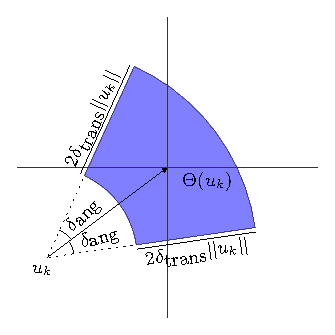
\includegraphics[scale=1.2]{figs/noisemodel}
    \caption{The noise model $\Theta(u_k)$ involves bounded angular error
      $\delta\sub{ang}$ and bounded translational error
      $\delta\sub{trans}||u||$.}
    \label{fig:noiseModel}
  \end{figure}	

\item \emph{Observation space} $Y$: an observation at stage $k$ is the sensor
  information collected by the robot, denoted as $y_k \in Y$.
\item \emph{Observation function} $h : X \to \pow(Y) $: we use a set-valued
  function to model the robot's observations, the set-valued nature of this function reflects
  that the sensing in our problem formulation can not be fully predicted. Also
  define a function
  \begin{equation}
    \label{eq:preimage}
    H(y_k) = \left\{ x_k \in X \mid y_k \in h(x_k), y_k \in Y \right\},
  \end{equation}
  in order to retrieve the set of states from which a given observation might be obtained.
\item \emph{Initial condition} $\eta_0$: initially we assume that we know a set
  $\eta_0$ containing all possible starting states of the robot, namely,
  $\eta_0$ represents a set $X_1\subseteq X$. 
\end{enumerate}

%\clearpage
\section{Information Space}
\label{sec:ispace}
The problem we address here is in a scenario in which the robot is able to complete
tasks without knowing the exact states. 
%
Therefore, the planning algorithm can be considered in terms of the information space respective.  
%
The ultimate objective of our approach is to form a plan $\pi$ which the robot can execute using the
information available in the information space.
%
Generally, an information space is essentially a special state space which involves the history of action and sensor observation. 
%
Here we follow the convention from LaValle's book~\cite{Lav06}. 
%
Assuming at every stage robot collects sensor observations and makes an action. 
The sensor history at stage $k$ is
\begin{equation}
  \label{eq:sensor-hist}
  \tilde{y}_k = (y_1, y_2, \ldots, y_k).
\end{equation}
The action history at stage $k$ contains every action from when the first action
was applied to the time when the latest action $u_{k-1}$ was applied. 
Thus, we have
\begin{equation}
  \label{eq:action-hist}
  \tilde{u}_{k-1} = (u_1, u_2, \ldots, u_{k-1}).
\end{equation}

\begin{defn} 
  A state $x_k \in X$ is \emph{consistent with} a sensor-action history
  $(\tilde{y}_k, \tilde{u}_{k-1})$ if there exists some state sequence
  $x_1,\ldots,x_{k+1} \in X$ such that $x_1 \in \eta_0$, and $x_{i+1} \in F(x_i,
  u_i)$ for each $i=1,\ldots,k$, and $y_i \in h(x_i)$ for each $i=1,\ldots,k+1$.
\end{defn}


\begin{defn}
  \label{def:istate} 
  The \emph{information state} (I-state) $\eta_k$ at stage $k$ is the set of all
  states consistent with the robot's sensor-action history.
\end{defn}


We can compute the history
I-state by combining the sensor-action history with the initial condition.
%
Denote the history I-state at stage $k$ using $\eta_k$, we have
\begin{equation}
  \label{eq:hist-istate}
  \eta_{k+1} = (\eta_0,\tilde{u}_{k},\tilde{y}_{k}).
\end{equation}
%
We noticed that the history I-state at stage $k+1$ contains all the information from
I-state at $k$ plus the latest observation $y_{k+1}$ and most recently applied
action $u_{k}$, we can write $\eta_{k+1}$ as
\begin{equation}
  \label{eq:hist-istate2}
  \eta_{k+1} = (\eta_{k}, {u}_{k}, y_{k+1}).
\end{equation}

\begin{defn}
  \label{def:ispace} 
  The \emph{information space} (I-space) $\Ispace$ is the
  powerset of $X$, which contains all possible I-states.
\end{defn}


Since the exact state $x_k$ is known to be contained in the I-state $\eta_k$, we
let $X(\eta_k) \subseteq X$ be the minimal subset in the state space consisted
with $\eta_k$. 
%
Recall Equation~\ref{eq:preimage}, we could infer the possible states from sensor observation $y_k$, $X_k(\eta_k) \subseteq H(y_k)$. 
%
Thus, starting from the initial condition, the robot updates its knowledge of 
possible states in terms of the history of its actions and observations. 


The base case for stage $1$ is formulated as:
\begin{equation}
  \label{eq:initial-istate}
  X_1(\eta_1) = X_1(\eta_0, y_1) \cap H(y_1).
\end{equation}
%
Assume that $X_k(\eta_k) \subseteq X$, $X_{k+1}(\eta_{k+1})$ can be inductively
computed. 
Recall Equation~\ref{eq:hist-istate2}, we have $\eta_{k+1} =
(\eta_{k}, {u}_{k}, y_{k})$, such that
\begin{equation}
  X_{k+1}(\eta_{k+1}) = X_{k+1}(\eta_{k}, {u}_{k}, y_{k}).
\end{equation}
%
Then we apply two set operations to compute the state subset
$X_{k+1}(\eta_{k+1})$: 
\begin{enumerate}
\item apply set union with the output of state transition function (Equation~\ref{eq:state-trans}) on every possible states contained in $X(\eta_k)$, we yield:
\begin{equation}
  X_{k+1}(\eta_{k}, u_k) =  \bigcup_{x_k \in \eta_k} F(x_k, u_k);
\end{equation}
\item apply set intersection on the observation preimage at stage $k$ with the
state subset from the first step:
\begin{equation}
  \eta_{k+1} = X_{k+1}(\eta_{k}, u_k) \cap H(y_{k}).
\end{equation}
\end{enumerate}
%
Hence, $\eta_{k+1}$ can be iteratively computed from starting condition
(Equation~\ref{eq:initial-istate}) using Equation~\ref{eq:istate-trans}:
\begin{equation}
  \label{eq:istate-trans}
  \eta_{k+1} =
  \left[ \bigcup_{x_k \in \eta_k} F(x_k, u_k) \right].
  \cap H(y_{k}).
\end{equation}


Use the computed I-state, the robot can make decision on its action in order to
complete the task, so that the plan $\pi: \Ispace \to U$, $u_k = \pi(\eta_k)$.

%\clearpage
\section{Range Space}
\label{sec:rspace}
The updates of the information state is computationally expensive since each
I-state contains many states and sensor-action history. 
%
To simplify the representation of the I-state $\eta_k$, our approach maintains only an
over-approximation of the $\eta_k$, denote as $A_k$, so that
\begin{equation}
  \eta_k \subseteq A_k.
\end{equation}
%
The key idea of our approximation approach is to select a range space $\Rspace
\subseteq \Ispace$ within the I-space, and constrain the approximated I-space to
remain a member of this range space, so that $A_k \in \Rspace$.
\begin{defn}
  \label{def:rspace}
  A range space $\Rspace \subseteq \Ispace$ is a set of I-states, equipped with
  two functions:
  \begin{enumerate}
  \item an \emph{approximate action update function} $T: \Rspace \times U \to
    \Rspace$, such that if $\eta_k \subseteq A_k$, then
    \begin{equation}
      \label{eq:T}
      \bigcup_{x_k \in \eta_k} F(x_k, u_k) \subseteq T(A_k, u_k);
    \end{equation}
  \item an \emph{approximate observation update function} $O: \Rspace \times
    Y \to \Rspace$, such that if $\eta_k \subseteq A_k$, then
    \begin{equation}
      \label{eq:O}
      \eta_k \cap H(y_k) \subseteq O(A_k, u_k).
    \end{equation}
  \end{enumerate}
\end{defn}
%
Similar to the information space, the approximation set $A_{k+1}$ containing the
I-state $\eta_k$ in the range space can be iteratively computed from an initial
state $A_0 = \eta_0$:
\begin{equation}
  A_{k+1} = O(T(A_k, u_k), y_{k}).
\end{equation}
%
We have used different types of geometric sets to approximate the I-state. 
%
The intuition is that we can use simple data structures to save all possible states
$x_k$ contained in the exact I-states such that $x_k \in A_k$.

\subsection{Disk Range Space}
\label{subsec:disk}
First we consider a circular approximation of the true I-state. 
%
In view of the computational efficiency, a circle or planar disk can be quickly parameterized
by a center point and a radius. 
%
Denote the set of all disks in $\Real^2$ using $\Rdisk$. 
Recall in a 2D plane, an information state can be represented using a compact set, 
thus, for any compact set $S \subset \Real^2$, let $\sed(S)$ denote the smallest disk enclosing $S$.
%
Then we define
\begin{flalign}
  \label{eq:tdisk} 
  T\disk(A_k, u_k) = A_k \oplus \{ u_k \}
  \oplus \sed(\Theta(u_k)).
\end{flalign}
%
In Section~\ref{sec:robot-mod}, we have mentioned that the action and
noise models in this problem are under addictive operation.
%
Hence, for two sets of pointer vectors, we apply the Minkowski sum operation~\cite{DebVanOveSch97}, denoted
using operator $\oplus$. 
%
Computing Minkowski sums of disks consists of the addition of their centers and radius, therefore, it takes constant time to compute $T\disk$.  
%
When the observation preimages are quarter-planes or circles, 
computing the $O\disk$ also takes constant time~\cite{OKa08b, OKaXu12}.
%  
Because both $A_k$ and $\sed(\Theta(u_k))$ are disks, the result is still in $\Rdisk$.  
%
Similarly, we define
\begin{equation} 
  O\disk(A_k, y_{k}) = \sed(H(y_{k}) \cap A_k).
\end{equation} 
It is trivial to show that $\Rdisk$ is a range space under the
operations of the action update and the observation update by definition.

\subsection{Rectangle Range Space}
\label{subsec:rect}
Denote an axis-aligned rectangle approximation set as $\Rrect \subset \Real^2$, 
each set can be simply represented by its lower left corner $a$ and
its upper right corner $b$. 
%
Similar to the $\sed$ operation in the $\Rdisk$, we define an operation to find the minimum axis-aligned rectangle given a compact set $S \subset \Real^2$.
We name the operation $\aabb(S)$, short for ``axis-aligned bounding box.''
%
Then, we can define
\begin{flalign}
  \label{eq:trect} 
  T\rect(A_k, u_k) = 
  \aabb(X\free \cap [A_k \oplus \{u_k\} \oplus \aabb(\Theta(u_k))]).
\end{flalign} 
%
Also we define the approximate observation update function:
\begin{equation}
  \label{eq:orect} 
  O\rect(A_k, y_{k}) = \aabb(H(y_{k}) \cap A_k).
\end{equation} 
%
By definition, we can show that $\Rrect$ is a range space under $T\rect$ and $O\rect$.

Figure~\ref{fig:rect-update12} and Figure~\ref{fig:rect-update34} illustrate the steps to
compute the approximation set $A_{k+1}$ using the approximate transition function $T\rect$ in the rectangle range space, as described in Equation~\ref{eq:trect}.

\begin{enumerate}
\item Step 1: find the minimal axis-aligned bounding box for the bounded noise set
  $\Theta(u_k)$ of action $u_k$, $\aabb(\Theta(u_k))$. 
  Since the set $\Theta(u_k)$ is represented as a list of vertices on its boundary, this
  operation takes linear time to find the extremal coordinates in each direction
  from the vertex list.

\item Step 2: compute the Minkowski sum $A_k \oplus \{ u_k \} \oplus \aabb(\Theta(u_k))$, 
  using the result of Step 1. 
  This step takes constant time because each of the three operands is either a single point or a rectangle
  represented by its lower left and upper right corners, the results can be
  computed by adding the coordinates of the respective corners together.
	
\item Step 3: intersect the free state space $X\free$ with the result of Step
  3, using the general polygon clipping algorithm~\cite{Vat92}. 
  This step yields a polygonal region that contains $\eta_k$.

\item Step 4: apply the same algorithm in Step 1 to find the axis-aligned
  bounding box of the result of Step 3. 
  Hence, we assure that the computed approximation set $A_{k+1} \in \Rrect$.
\end{enumerate}
\begin{figure}
\centering
  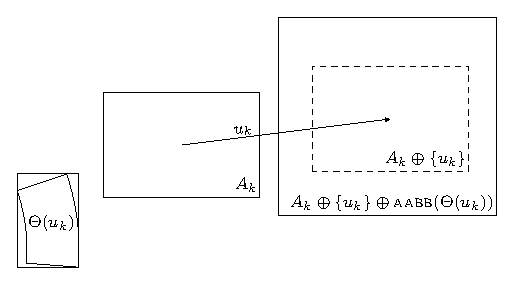
\includegraphics[scale=1.2]{figs/rect-update2}  
  \caption{Steps 1 and 2 of proceeding approximate observation update function}
  \label{fig:rect-update12}
\end{figure}

\begin{figure}
  \centering
  \begin{minipage}[b]{0.45\linewidth}
    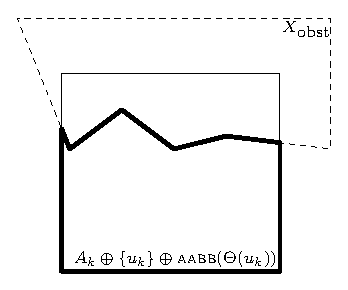
\includegraphics[scale=1.25]{figs/rect-update3}% \\  \hfill
  \end{minipage}
  \bigskip
  \begin{minipage}[b]{0.45\linewidth}
    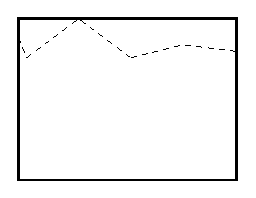
\includegraphics[scale=1.25]{figs/rect-update4}
  \end{minipage}
  \caption{Steps 3 and 4 of proceeding the approximate action update function}
  \label{fig:rect-update34}
\end{figure}

According to Equation~\ref{eq:orect}, the approximation set can be updated with
the observation preimage. 
%
We let the observation preimage be a disk in $\Real^2$, the intuition is to accelerate the computation by modeling the preimage using a specific known shape, such as disk or other geometric shapes. 
%
In our experiments, every $H(y_k)$ is modeled using a planar disk.  
In that case, we can compute $O\rect(A_k, y_k)$ in constant time using following
steps (Figure~\ref{fig:orect}): 
\begin{enumerate}
\item Step 1: compute the set of points at which the boundary of the disk
  $H(y_{k})$ intersects the boundary of the rectangle $A_k$. 
  There are at most $8$ such points.
  
\item Step 2: for each of four axis-aligned extremal points of the disk
  $H(y_{k}),$ that is, its topmost, bottommost, leftmost, and rightmost
  points, check if it is a subset in $A_k$.

\item Step 3: find the minimum axis-aligned rectangle that contains the
  8 or fewer points found in Steps~1 and 2.
\end{enumerate}

\begin{figure} 
  \centering
  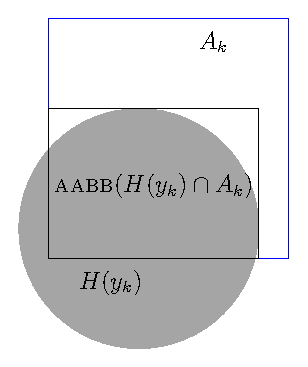
\includegraphics[scale=1]{figs/circlerect}
  \caption{Computing $O\rect(A_k, y_{k})$ to find the rectangle approximated I-state, 
    given an observation $y_{k}$.}
  \label{fig:orect}
\end{figure}

\subsection{Double-Rectangle Range Space}
\label{subsec:dblrect}
Using the geometric shapes, such as disk, or rectangle, to
approximate the I-state limits to provide good approximations
when the exact I-state $\eta_k$ is not a convex set. 
That is, the over-approximation set could be far from close to the true I-state in this case.

To overcome this limitation, our work contributes to a novel range space,
\emph{double-rectangle}, which is essentially a union of two rectangular
regions, for both convex and non-convex I-states over-approximation:
\begin{equation}
  \Rdrect = \{ R_1 \cup R_2 \mid R_1, R_2 \in \Rrect \}.
\end{equation}

To make the new range space useful, we have to define a function that enforces the $\Rdrect$ 
to be a range space under operations of the action transition (Equation~\ref{eq:T}) 
and the observation update (Equation~\ref{eq:O}).

We introduce an algorithm called $\drap$, short for the term ``double rectangle
around polygon'', which accepts a polygonal region in $\Real^2$ as input, and
outputs a small double-rectangle containing that polygon.  
%
The intuition of this algorithm is to maintain the size of the resulting double-rectangle as small
as possible, but not necessarily minimum in view of the computation efficiency.

\begin{figure} 
  \centering
  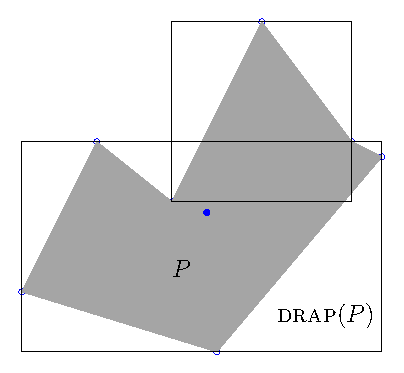
\includegraphics[scale=1]{figs/doublerect}
  \caption{A double-rectangle around the given a non-convex input polygon $P$}
  \label{fig:drap}
  %}
\end{figure}

Figure~\ref{fig:drap} shows an example of the executing the Algorithm~\ref{alg:drap}. 
%
The $\drap$ algorithm uses a bottom-up manner to find the double rectangle. 
%
Starting with two degenerate rectangles, each one is a single point at either a vertex of the polygon or at its centroid, as ``seeds''.
%
Then an iterative process considers each edge of the polygon in turn, and
expands one of the two rectangles to contain that edge.  
%
In each iteration, we choose between the two possible expansions by greedily preferring the rectangle
to expand that results in the smallest total area.  
%
Finally, to ensure that the result does not contain any unnecessary over-approximation, 
we repeat this process over all pairs of potential seed points, and retain only the smallest
overall double rectangle, as measured by its area. 
%
For a polygon with $n$ vertices, this algorithm takes $O(n^3)$ time.
% 
The outer loop runs $O(n^2)$ times since there are $C_n^2$ pairs of vertices, in
which $C_n^2$ is a binomial coefficient. The inner loop runs $O(n)$ times.

With the Algorithm~\ref{alg:drap}, we show that $\Rdrect$ is in a range space by definition.
%
For a double-rectangle I-state approximation $A_k = R_1 \cup R_2$, we have
\begin{flalign}
  \label{eq:dblrect-T}
  T\drect(A_k, u_k) = \drap(X\free \cap [A_k \oplus \{ u_k \} \oplus
  \drap(\Theta(u_k))]), \\
  O\drect(A_k, y_{k}) =  \aabb(H(y_{k}) \cap R_1)
  \cup \aabb(H(y_{k}) \cap R_2).
\end{flalign}

\begin{algorithm}
    \SetKwInOut{Input}{input}
    \SetKwInOut{Output}{output}
    \Input{A polygon $P$}
    \Output{A double-rectangle over-approximating $P$}
    $V \leftarrow $ a set containing the vertices of $P$ and its centroid\;
    $C \leftarrow $ a set containing double-rectangle approximations\;
    \ForEach {vertex pair $p,q \in V, p \neq q$}{
        $R_1 \leftarrow \{ p \}$; $R_2 \leftarrow \{ q \}$\;
	    \ForEach {edge $e \in P$}{
		    $R_1' \leftarrow$ $\aabb(R_1 \cup e)$\;
		    $R_2' \leftarrow$ $\aabb(R_2 \cup e)$\;
		    \eIf{$\area(R_1' \cup R_2) < \area(R_1 \cup R_2')$}{
		        $R_1 \leftarrow R_1'$\;
		    }{
		        $R_2 \leftarrow R_2'$\;
		    }
	    }
	    insert $R_1 \cup R_2$ into $C$\;
	}
    \Return
    $\operatornamewithlimits{argmin}_{(R_1 \cup R_2) \in C}(\area(R_1 \cup R_2))$\;
    \caption{Compute a double-rectangle approximation of a polygon}
    \label{alg:drap}
\end{algorithm}

%\clearpage
\section{Performance Evaluation}
\label{sec:simu-cga}
To evaluate the quality of the approximation throughout the robot's execution,
we can compare the area of the approximated I-state to the area of the
I-state itself:
\begin{equation}
  \label{eq:error}
  Q_k = \frac{1}{k} \sum_{i=1}^k \frac{\area(\eta_i)}{\area(A_i)}.
\end{equation}
The higher value of $Q$ demonstrates the better approximation quality, up to
a maximum value of $1$. 


\subsection{Navigation Task}
\label{subsec:nav}
One application of our method is that the robot can form a plan without
requiring to know its exact state in a landmark-based navigation task.  
%
In a known environment with or without obstacles, we placed landmarks in the
locations of $l_1,\ldots,l_m$ which can be detected by the robot. 
%
Each landmark has an detection range $\range_i, i \in [1, \ldots, m]$, therefore, the observation
preimage is a disk with center point at $l_i$ and radius $\range_i$. 
%
Moreover, to navigate the robot, we place a sequence of waypoints $w_1,\ldots,w_n$
such that each waypoint is visible and reachable 
by the robot from both its predecessor and its successor.

In order to complete the navigation task, the robot needs to form a plan of
sequentially visiting each of the waypoints, by utilizing the imperfect sensed
information and its noise movements. 
%
We consider a robot has successfully completed a task if and only if the robot finished visiting the waypoints in finite time. 
%
Otherwise, we consider the failure of a task if the robot collides with
an obstacle or it takes too long time to reach the final waypoint.

We denote the next waypoint by $w$ and select an action that moves toward $w$
from the centroid of $A_k$ in terms of plan $\pi(A_k)$:
\begin{equation}
  \label{eq:vhat}
  \pi(A_k) = \dfrac{w - \operatorname{centroid}(A_k)}{\|w- \operatorname{centroid}(A_k)\|} v\sub{max}.
\end{equation}

\subsection{Experimental Results}
\label{subsec:exp}
To verify the effectiveness and efficiency of CGA for the navigation task, we
conducted experiments using three distinct environments
(Figure~\ref{fig:env}), and three distinct range spaces: $\Rspace_{disk}$,
$\Rspace_{rect}$, and $\Rspace_{dblrect}$.  
%
We implemented the experiments using C++, and performed all the simulations on a GNU/Linux PC with Intel Core i7 CPU, 2.8GHz and 8GB memory.
We present experiments that measured these approximation ratios, 
along with the robot's success rate in completing the navigation task using each of these range spaces.
\begin{figure}
  \centering
  \begin{minipage}[b]{0.45\textwidth}
    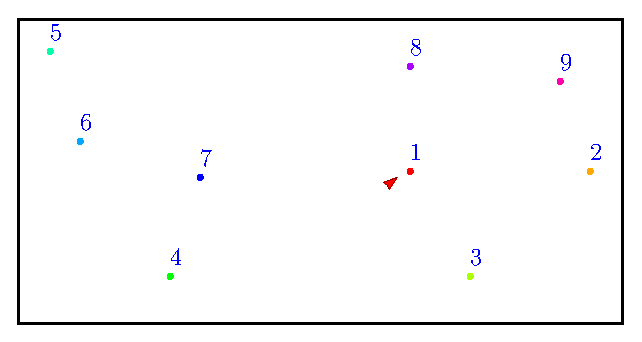
\includegraphics[scale=0.65]{figs/blank}  \\ 
    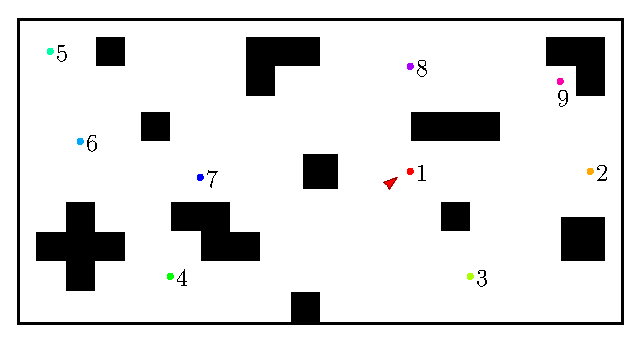
\includegraphics[scale=0.65]{figs/clutter}  
  \end{minipage}
  \begin{minipage}[b]{0.45\textwidth}
    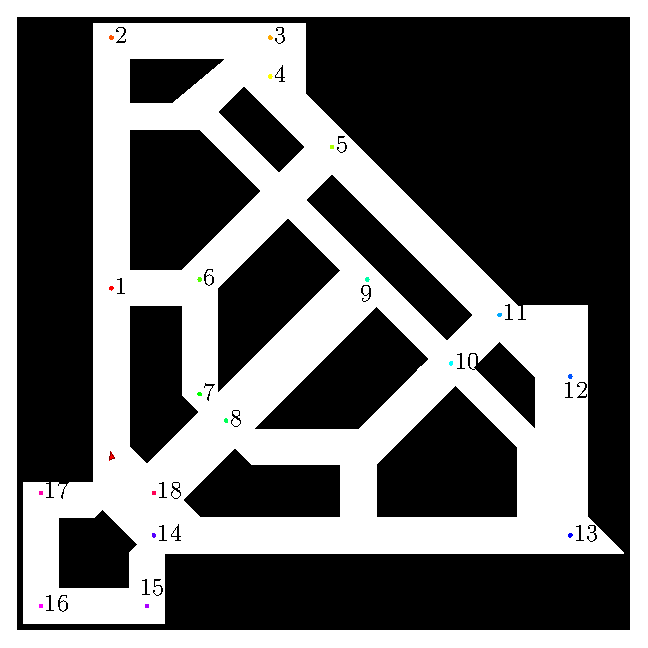
\includegraphics[scale=0.65]{figs/office}    
  \end{minipage}
  \caption{Three environments with landmarks: [top left] Obstacle-free. [bottom
    left] Obstacle-clutter. [right] Office-like.}
  \label{fig:env}
\end{figure}

\subsubsection{Task Completion Using CGA}
In each environment, we performed two series of experiments. 
%
First, we varied the number of landmarks $N$ between $5$ and $250$ in increments of $5$ and calculated the
robot's success rate.  
%
For each $N$, we repeated the experiment $15$ times with different landmark distributions generated from distinct random seeds. 
%
The success rate is the number of times that task completes successfully divided by
the total number of trials.  
%
Figures~\ref{fig:sucRate1}, \ref{fig:sucRate2}, and \ref{fig:sucRate3} show the average success rate for three environments, respectively. 
%
We conclude that using the approximated I-states can achieve similar performance as using the true I-state, 
especially when using $\Rrect$ and $\Rdrect$.

\begin{figure}
  \begin{center}
    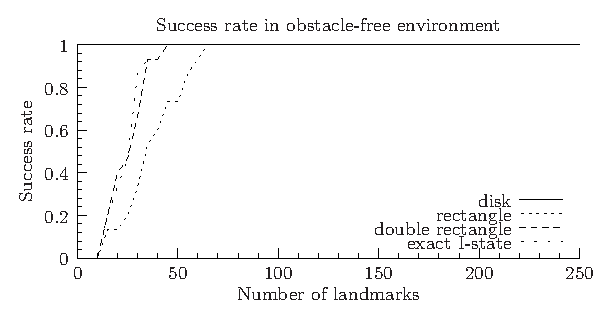
\includegraphics[width=0.95\textwidth]{figs/exp_num_blank}
  \end{center}
  \caption{The statistics of the success rate versus 
    the number of landmarks in the obstacle-free environment.}
  \label{fig:sucRate1}
\end{figure}
\begin{figure}
  \begin{center}
    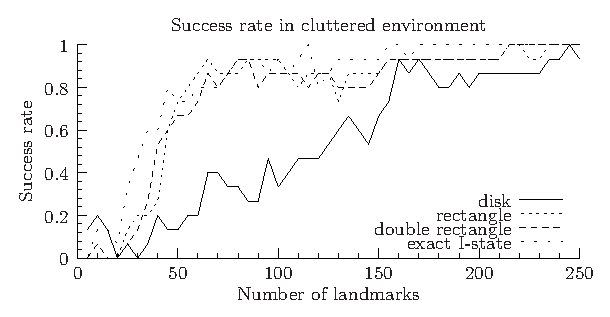
\includegraphics[width=0.95\textwidth]{figs/exp_num_clutter}
  \end{center}
  \caption{The statistics of the success rate versus 
    the number of landmarks in the obstacle-cluttered environment.}
  \label{fig:sucRate2}
\end{figure}
\begin{figure}
  \begin{center}
    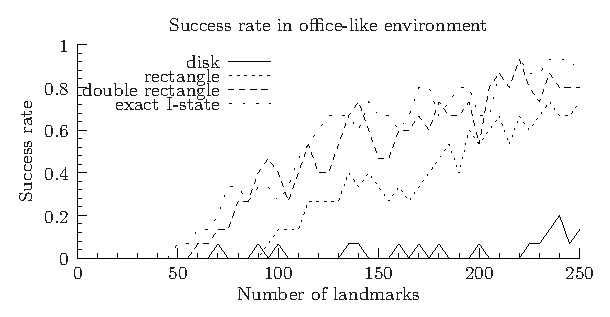
\includegraphics[width=0.95\textwidth]{figs/exp_num_cse}
  \end{center}
  \caption{The statistics of the success rate versus 
    the number of landmarks in the office-like environment.}
  \label{fig:sucRate3}
\end{figure}

Using $\Rdisk$ in the environments with obstacles yields the lowest success rate comparing to other range spaces. 
%
We conclude the reason as that $T\disk$ does not take the obstacles into account
(Equation~\ref{eq:tdisk}). 
%
We omit this step from $T\disk$ because computing $\sed$ for complex obstacle shapes is computationally expensive. 
%
The success rates of using three range spaces in the office-like environment
(Figure~\ref{fig:sucRate3}) are lower than the results in other
environments. 
%
The reason that directly impacts the performance is that there are more obstacles 
and narrow corridors in this environment. 
%
Meanwhile, after comparing the success rates of using different range spaces in the same environment, 
we conclude that using the double-rectangle approximated I-states provides better
performance over using the other types of range spaces.


Moreover, we conducted experiments to evaluate the impact of the selection of axes. 
%
Consider both $\Rrect$ and $\Rdrect$ range spaces, they are constructed based on only
axis-aligned rectangles. 
Therefore, we have comprehensively evaluated the performance of the CGA method by performing these experiments below.
%
We rotated each environment for a degree between $0$ and $2\pi$ radians, in increments of $\pi/12$, 
and executed $10$ trials with $250$ landmarks in each environment.
%
Figures~\ref{fig:sucRate4} and \ref{fig:sucRate5} show the success rates of
using three range spaces in two environments with obstacles. 
%
We omit the results for the obstacle-free environment here since the robot always accomplished the
navigation task in each trial. 
%
Above all, the results have demonstrated that there is no substantial degradation 
of CGA's performance as a function of environment rotation.


\begin{figure}
  \begin{center}
    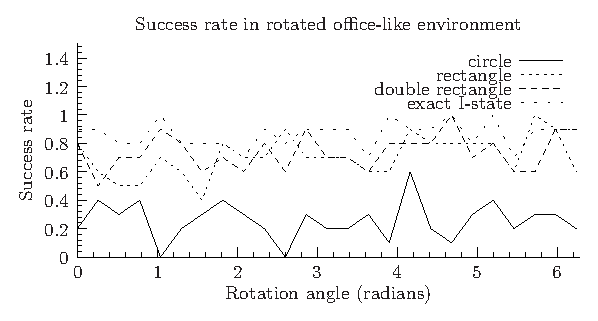
\includegraphics[width=0.95\textwidth]{figs/exp_rot_cse}
  \end{center}
  \caption{The statistics of the success rate versus 
    the number of landmarks in the rotated office-like environment.}
  \label{fig:sucRate4}
\end{figure}

\begin{figure}
  \begin{center}
    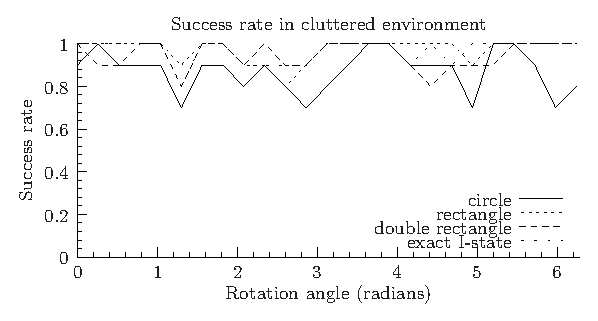
\includegraphics[width=0.95\textwidth]{figs/exp_rot_clutter}
  \end{center}
  \caption{The statistics of the success rate versus 
    the number of landmarks in the rotated obstacle-clutter environment.}
  \label{fig:sucRate5}
\end{figure}

\subsubsection{Computation Time and Approximation Quality}

We also conducted experiments to compare the computation time of our approximated
I-states with the corresponding computation time of the exact I-states.  
%
We used $N=300$ landmarks and conducted $10$ trials for each combination of the range space
and the environment.  
%
At the same time, we compute the approximation ratio $Q$ as defined in Equation~\ref{eq:error}.  
%
From the results shown in Table~\ref{tab:exp-data}, 
we conclude that there is a trade-off between the computation time and the approximation quality of using different range spaces. 
%
Moreover, the results demonstrate that using the double-rectangle range space could produce the highest approximation quality.

\begin{table}
  \small\centering
  \caption{Experimental results: computation time and approximation
      ratio for range spaces and I-space in three testing environments.}
    \begin{tabular}{ccccccc} 
    \toprule 
    \textbf{Range}  & \multicolumn{2}{c}{\textbf{Obstacle-free}} & \multicolumn{2}{c}{\textbf{Clutter}} & \multicolumn{2}{c}{\textbf{Office-like}}\\
    \textbf{Space} & \textbf{Time(s)} & \textbf{Approx.Ratio} & \textbf{Time(s)} & \textbf{Approx.Ratio} & \textbf{Time(s)} & \textbf{Approx.Ratio} \\
    \midrule
    $\Rspace_{disk}$ & 0.163 & 0.155 & 0.162 & 0.155  & 0.292 & 0.220 \\ 
    \midrule
    $\Rspace_{rect}$ & 0.396 & 0.642  & 0.441 & 0.632 & 0.415 & 0.661 \\
    \midrule
    $\Rspace_{dblrect}$ & 1.021 & 0.684 & 1.122 & 0.691 & 1.491 & 0.720 \\
    \midrule
    $\Ispace$ & 10.074 & 1.000 & 10.218 & 1.000 & 26.895 & 1.000 \\
    \bottomrule     
    \end{tabular}
    \label{tab:exp-data}
\end{table}


The results of these experiments have verified the effectiveness of our over-approximating approach.
%
Specifically, the innovation of the range space as the union of
two rectangles improves the approximation accuracy. 
%
We conclude that our method of representing a robot's uncertainty and reasoning about its state is useful 
for robot to complete specific tasks, such as navigation task based on the landmarks, even subject to a low approximation ratio.

However, it remains as future work to consider additional range spaces.  
%
Particularly, we can extend this approach to a general method to approximate the exact I-state using $k$-fold unions of rectangles, 
without any substantial changes to the algorithm.  

We can expect the trade-offs between accuracy and efficiency that are exposed by using
larger numbers of rectangles in the approximated I-state.  

Furthermore, the range spaces that allow more general polygonal shapes are worthy to be considered. 
The challenge is how to maintain efficiency by limiting their number of vertices, 
and by applying appropriate expansion operations to enforce this limit.



